\begin{problem}{${problem.name}}<#--
-->{<#if "stdin" == problem.inputFile><#--
     --><#if "russian" == language>стандартный ввод<#--
     --><#else>standard input<#--
     --></#if><#else>${problem.inputFile}</#if>}<#--
-->{<#if "stdout" == problem.outputFile><#--
     --><#if "russian" == language>стандартный вывод<#--
     --><#else>standard output<#--
     --></#if><#else>${problem.outputFile}</#if>}<#--
--><#assign timeLimit=problem.timeLimit/1000/><#--
--><#if language="russian"><#--
    --><#if problem.timeLimit%1000!=0||(10<=timeLimit%100&&timeLimit%100<20)||timeLimit%10=0||5<=timeLimit><#--
        -->{${timeLimit?c} секунд}<#--
    --><#else><#--
        --><#if timeLimit%10=1><#--
            -->{${timeLimit?c} секунда}<#--
        --><#else><#--
            -->{${timeLimit?c} секунды}<#--
        --></#if><#--
    --></#if><#--
--><#else><#--
    -->{${timeLimit?c} second<#if (timeLimit!=1)>s</#if>}<#--
--></#if><#--
--><#assign memoryLimit=problem.memoryLimit/1048576/><#--
--><#if language="russian"><#--
    --><#if problem.memoryLimit%1048576==0&&!(10<=memoryLimit%100&&memoryLimit%100<20)&&2<=memoryLimit%10&&memoryLimit%10<5><#--
        -->{${memoryLimit?c} мегабайта}
    <#else><#--
        -->{${memoryLimit?c} мегабайт}
    </#if>
<#else><#--
    -->{${memoryLimit?c} megabyte<#if (memoryLimit>1)>s</#if>}
</#if>

<#if providedStatementsCommands?? && providedStatementsCommands?size != 0><#--
    --><#list providedStatementsCommands as command><#--
        -->${command?string}
</#list>

</#if>
${problem.legend}

<#if problem.input?? && (problem.input?length>0)>
\InputFile
${problem.input}

</#if>
<#if problem.output?? && (problem.output?length>0)>
\OutputFile
${problem.output}

</#if>
<#if problem.interaction?? && (problem.interaction?length>0)>
\Interaction
${problem.interaction}

</#if>
<#if problem.scoring?? && (problem.scoring?length>0)>
\Scoring
${problem.scoring}

</#if>
<#if  (problem.sampleTests?size>0)>
\Example<#if  (problem.sampleTests?size>1)>s</#if>

\exmpthreewidinf=0.22\thelinewidth
\exmpthreewidouf=0.22\thelinewidth
\exmpthreewidnote=0.46\thelinewidth
\def\kwExampleNotes{Illustration}



\begin{examplethree}
<#list problem.sampleTests as test>
\exmp{${test.input}}{${test.output}}{
\vspace{-1mm}
\center
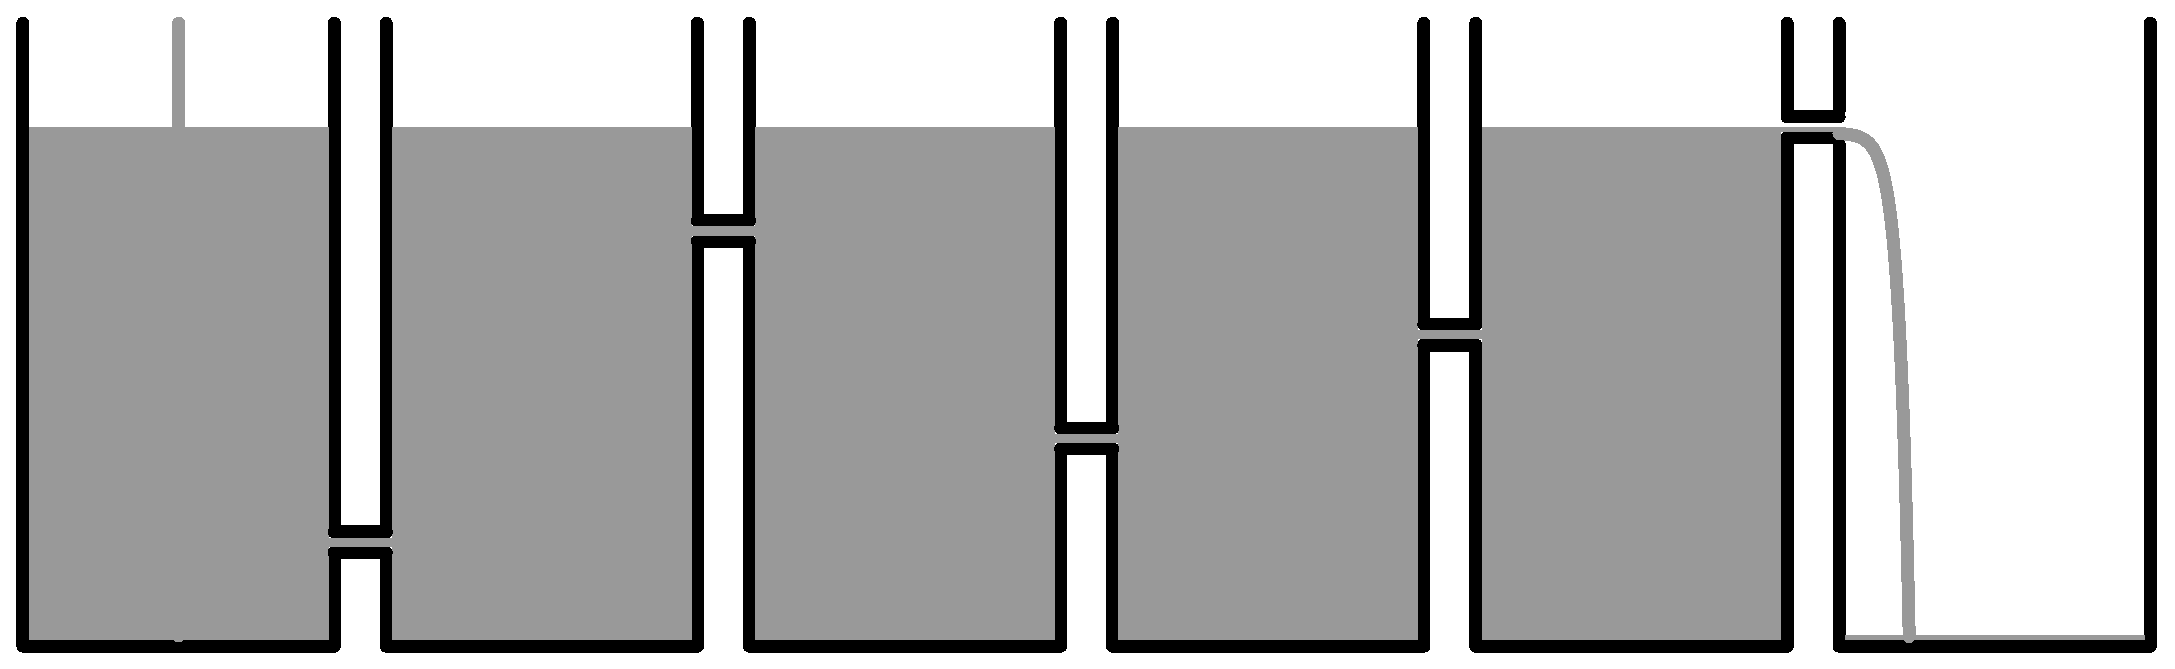
\includegraphics[scale=0.15]{joined-1.eps}
\vspace{2mm}
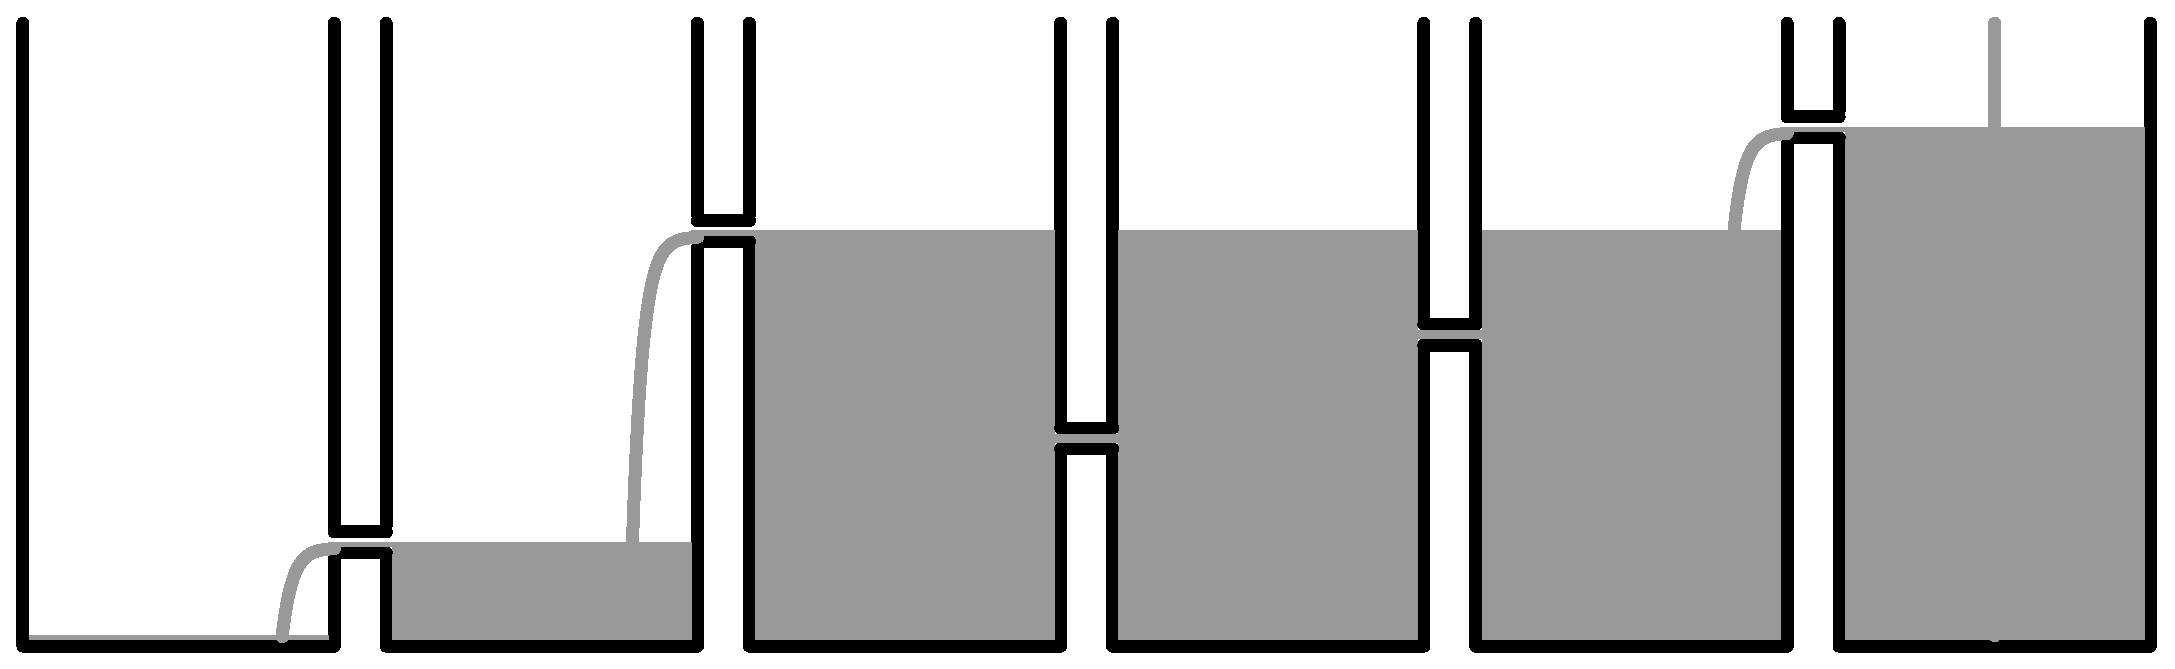
\includegraphics[scale=0.15]{joined-2.eps}
\vspace{2mm}
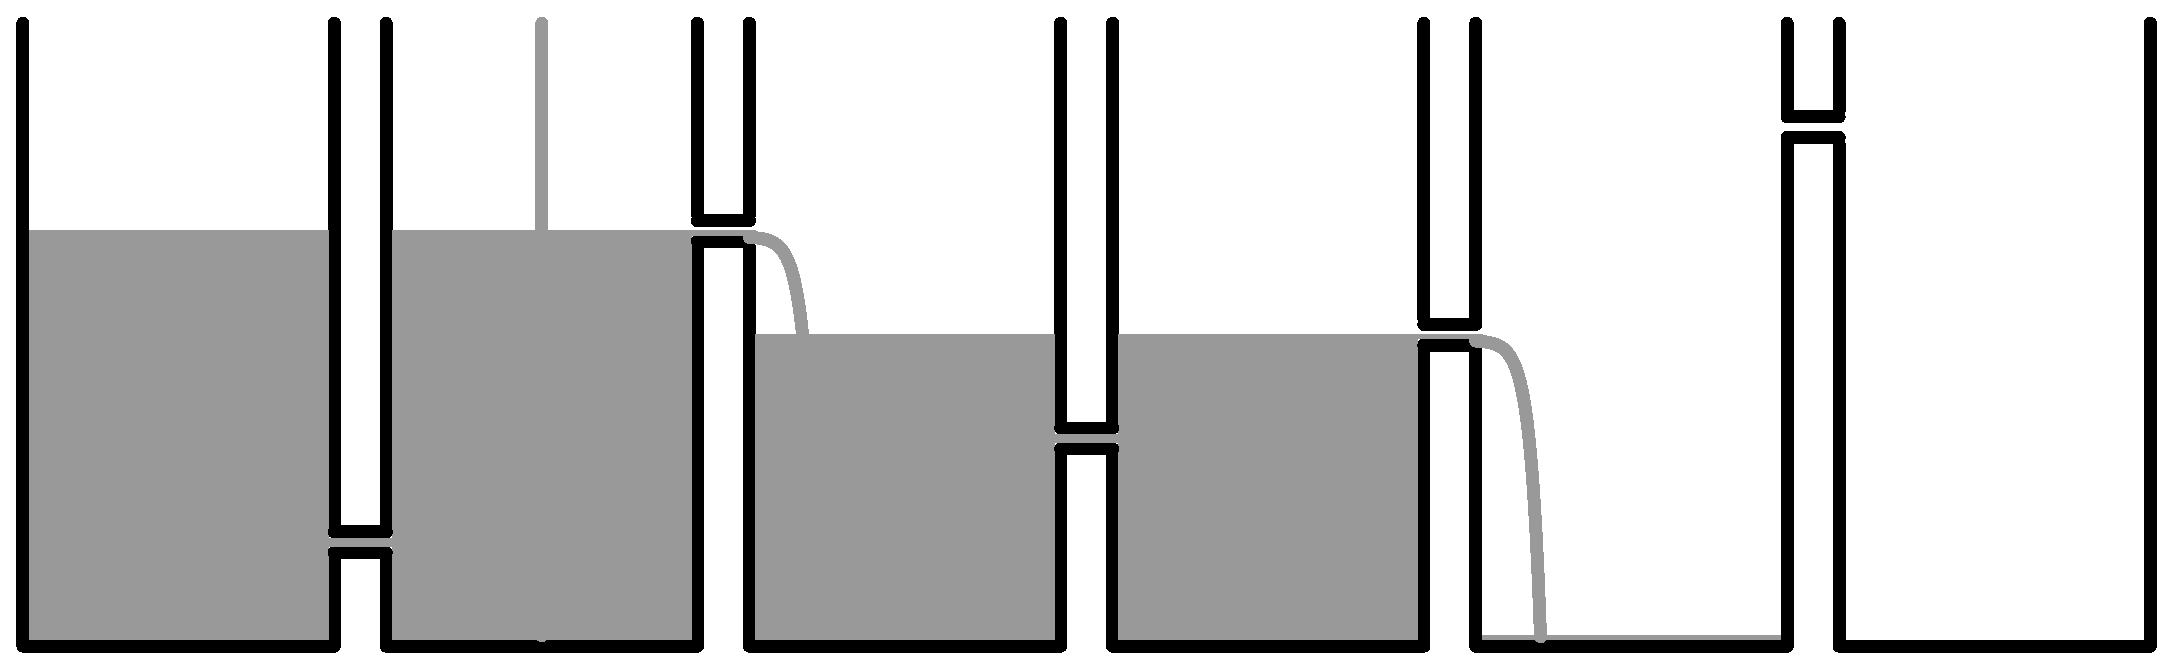
\includegraphics[scale=0.15]{joined-3.eps}
\vspace{2mm}
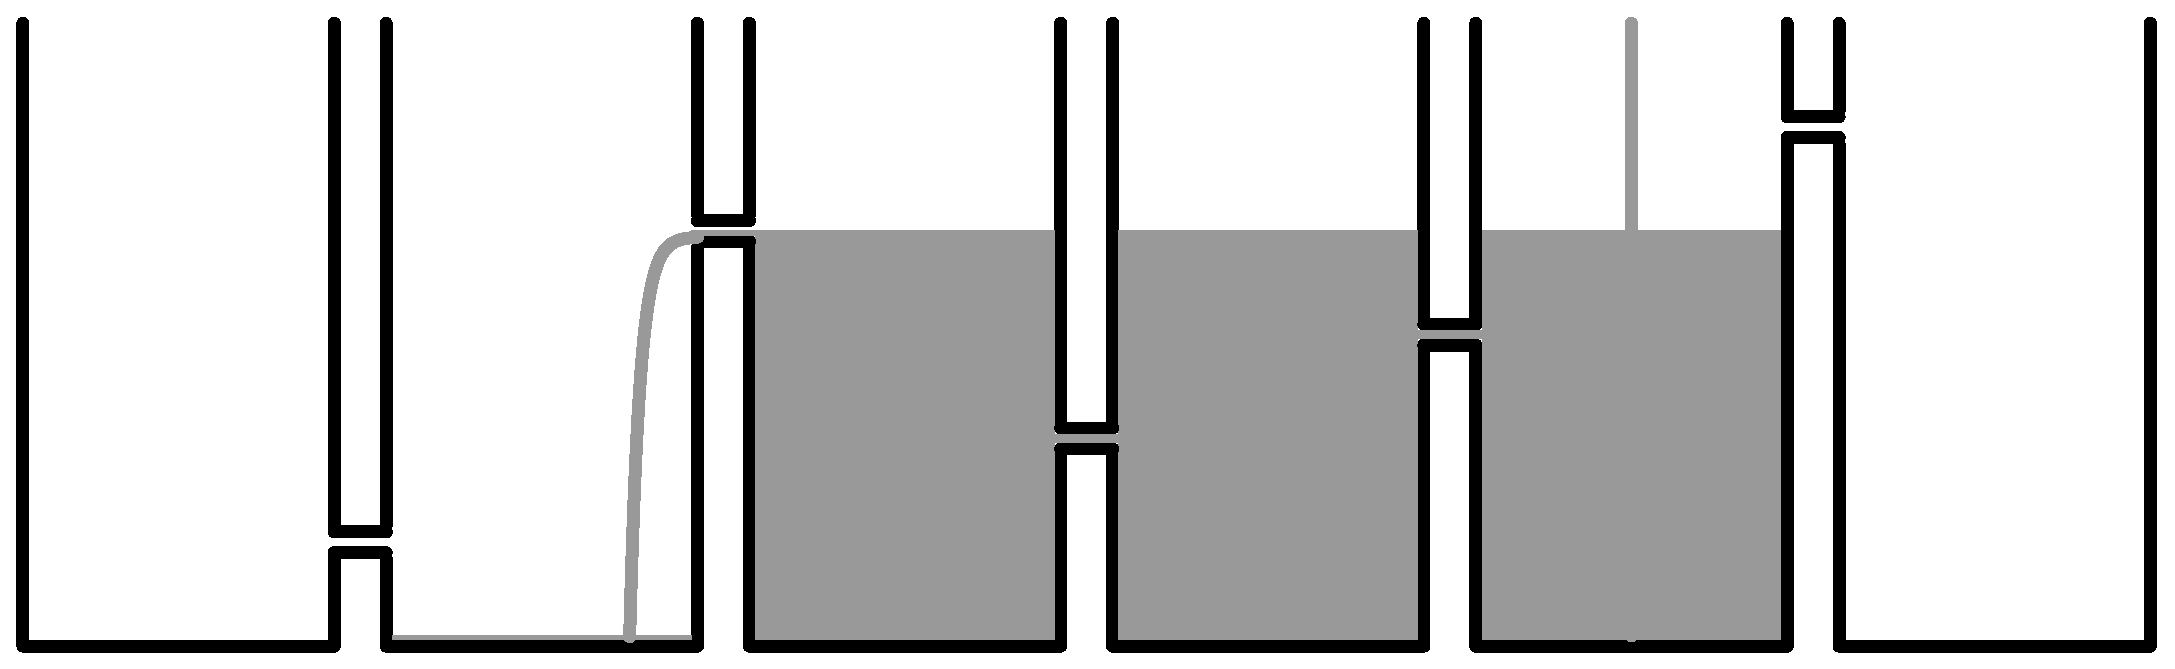
\includegraphics[scale=0.15]{joined-4.eps}
\vspace{2mm}
}%
</#list>
\end{examplethree}
</#if>

<#if (problem.notes??) && (problem.notes?length > 0)>
\Note
${problem.notes}

</#if>
\end{problem}

